% !TEX root = ../patchEmbeddings_review.tex


\section{Experiments on Neuron Segmentation}
\subsection{Data: CREMI Challenge} \label{sec:cremi_challenge}
We evaluate and compare our method on the task of neuron segmentation in electron microscopy (EM) image volumes. This application is of key interest in connectomics, a field of neuro-science with the goal of reconstructing neural wiring diagrams spanning complete central nervous systems. Currently, only proof-reading or manual tracing yields sufficient accuracy for correct circuit reconstruction \cite{schlegel2017learning}, thus further progress is required in automated reconstruction methods (see Fig. \ref{fig:MWS_segm} for an example of output neuron segmentation).

We test our method on the competitive CREMI 2016 EM Segmentation Challenge \cite{cremiChallenge} that is currently the neuron segmentation challenge with the largest amount of training data available. The dataset comes from serial section EM of \emph{Drosophila} fruit-fly brain tissue and consists of 6 volumes of $1250\times 1250\times 125$ voxels at resolution $4\times 4\times 40$ nm$^3$, three of which come with publicly available training ground truth. 
We achieved the best scores by downscaling the resolution of the EM data by a factor $(\frac{1}{2},\frac{1}{2},1)$, since this helped increasing the 3D context provided as input to the model.
We use the second half of CREMI sample C as validation set for our comparison experiments in Table \ref{tab:val_results} and then we train a final model on all the three samples with available ground truth labels to submit results to the leader-board in Tab. \ref{tab:test_results}. 
Results  are evaluated using the CREMI score, which is given by the geometric mean of Variation of Information Score (VOI split + VOI merge) and Adapted Rand-Score (Rand-Score), two popular metrics used to evaluate clusterings \cite{arganda2015crowdsourcing}.

\textbf{Data Augmentation} -- The data from the CREMI challenge is highly \linebreak anisotropic and contains artifacts like missing sections, staining precipitations and support film folds. 
To alleviate difficulties stemming from misalignment, we use a version of the data that was elastically realigned by the challenge organizers with the method of \cite{saalfeld2012elastic}.
In addition to the standard data augmentation techniques of random rotations, random flips and  elastic deformations, we simulate data artifacts.
In more detail, we randomly zero-out slices, introduce alignment jitter and paste artifacts extracted from the training data. Both \cite{funke2018large} and \cite{lee2017superhuman} have shown
that these kinds of augmentations can help to alleviate issues caused by EM-imaging artifacts. For zero-out slices, the model is trained to predict the ground-truth labels of the previous slice.
On the test samples, we run predictions for overlapping volumes and then average them.


 
 


\subsection{Architecture details of the tested models}\label{sec:models_details}
As a backbone model we use a 3D U-Net consisting of a hierarchy of four feature maps with anisotropic downscaling factors $(\frac{1}{2},\frac{1}{2},1)$, similarly to \cite{lee2019learning,lee2017superhuman,wolf2018mutex}. 
% U-Net with three levels in the feauter map hierarchy, involving downscaling factors $(1, \frac{1}{2},\frac{1}{2})$
Models are trained with the Adam optimizer and a batch size equal to one. Before applying the loss, we slightly crop the predictions to prevent training on borders where not enough surrounding context is provided. 
See Sec. \ref{sec:arch_details_suppl} and Fig. \ref{fig:model_architecture} in supplementary material for all details about the used architecture. 

 
\textbf{Baseline Model (SNB)} -- As a strong baseline, we re-implement the current state-of-the-art and train a model to predict affinities for a sparse neighborhood structure (Fig. \ref{fig:main_figure}a). We perform deep supervision by attaching three \emph{\sparseBr branches} (SNB) at different levels in the hierarchy of the UNet decoder and train the coarser feature maps to predict longer range affinities. Details about the used neighborhood structures and the architecture can be found in Table \ref{tab:neighborhood_structures} and Fig. \ref{fig:model_architecture}.

\textbf{Proposed Model (ENB)} -- We then train a model to predict encoded \maskname masks (Fig. \ref{fig:main_figure}c). Similarly to the baseline model, we provide deep supervision by attaching four \emph{\encBr branches} (ENB) to the backbone U-Net. As explained in Sec. \ref{sec:multiscale_patches}, all branches predict 3D masks of shape $7 \times 7 \times 5$, but at different resolutions $(1,1,1)$, $(\frac{1}{4},\frac{1}{4},1)$ and $(\frac{1}{8},\frac{1}{8},1)$, as we show in Fig. \ref{fig:model_architecture}.

\textbf{Combined Model (SNB+ENB)} -- Finally, we also train a combined model to predict both \maskname masks and a sparse neighborhood of affinities, by providing deep supervision both via \emph{\encBr} and \emph{\sparseBr} \emph{branches}. The backbone of this model is then trained with a total of seven branches: three branches equivalent to the ones used in the baseline model SNB, plus four additional ones like those in the ENB model (see Fig. \ref{fig:model_architecture}).  

\subsection{Graph Partitioning Methods} 
Given the predicted encoded \maskname masks, we compute affinities $a_e$ either with the average aggregation method introduced in Sec. \ref{sec:aggr_affs} (\textbf{MaskAggr}) or the efficient approach described in Sec. \ref{sec:efficient_affs}. 
The result of either is a signed pixel grid-graph, i.e. a graph with positive and negative edge weights that needs to be partitioned into instances. 
The used neighborhood connectivity of the graph is given in Table \ref{tab:neighborhood_structures}. Positive and negative edge weights $w_e$ are computed by applying the additive transformation $w_e=a_e-0.5$ to the predicted affinities.


To obtain final instances, we test different partitioning algorithms.
 % that have been already applied to neuron segmentation. 
The Mutex Watershed (\textbf{MWS}) \cite{wolf2018mutex} is an efficient algorithm to partition graphs with both attractive and repulsive weights without the need for extra parameters. It can easily handle the large graphs considered here with up to $10^8$ nodes/voxels and $10^9$ edges\footnote{Among all edges given by the chosen neighborhood structure, we add only 10\% of the long-range ones, since the Mutex Watershed was shown to perform optimally in this setup \cite{bailoni2019generalized,wolf2018mutex}.}. 

Then, we also test another graph partitioning pipeline that has often been applied to neuron segmentation because of its robustness. This method first generates a 2D super-pixel over-segmentation from the model predictions and then partitions the associated region-adjacency graph to obtain final instances. Super-pixels are computed with the following procedure: First, the predicted direct-neighbor affinities are averaged over the two isotropic directions to obtain a 2D neuron-membrane probability map; then, for each single 2D image in the stack, super-pixels are generated by running a watershed algorithm seeded at the maxima of the boundary-map distance transform (\textbf{WSDT}). Given this initial over-segmentation, a 3D region-adjacency graph is built, so that each super-pixel is represented by a node in the graph. Edge weights of this graph are computed by averaging short- and long-range affinities over the boundaries of neighboring super-pixels. 
Finally, the graph is partitioned by applying the average agglomeration algorithm proposed in \cite{bailoni2019generalized} (\textbf{GaspAvg}).

% GaspAverage is more robust to noise as compared to Mutex Watershed \cite{bailoni2019generalized}, but it is considerably more computationally expensive on large graphs like the ones considered here (up to $10^8$ nodes/voxels and $10^9$ edges). Thus, in our comparison on the validation set, we also... 

  





% \begin{figure}[t]
%         \centering
% \begin{minipage}[t]{0.49\textwidth}
%     \centering
%     % \scriptsize
%         \begin{tabular}[t]{l|c}
%          Method & \makecell{CREMI-Score \\(lower is better)} \\ \midrule 
% \textbf{} \textbf{Average}& \textbf{0.226}  \\
%  Sum + Constraints \cite{levinkov2017comparative} & 0.282 \\
%  Abs. Max. \cite{wolf2018mutex} & 0.322 \\
%  Max. + Constraints & 0.324 \\
%  Sum \cite{keuper2015efficient} & 0.334 \\
%  Average + Constraints & 0.563 \\
% THRESH & 1.521 \\ 
%         \end{tabular}
%     % \captionof{table}{CREMI-Scores achieved by different linkage criteria and thresholding. All methods use the affinity predictions from our CNN as input. Scores are averaged over the three CREMI training datasets.}
%     \label{tab:results_cremi_train}
% \end{minipage}\hfill
% % \begin{minipage}[t]{0.35\textwidth}
% % \centering
% %     \scriptsize
% %     \vspace*{-1.5em}
% % \begin{tabular}[t]{l|cc}
% %         \multirow{2}{*}{Method}    & AP  & AP 50\% \\ 
% %          & \multicolumn{2}{c}{(higher is better)} \\ \midrule
% %            Panoptic-DeepLab \cite{cheng2019panopticdeeplab} & 34.6 & 57.3 \\
% %            UPSNet \cite{xiong2019upsnet} $\dagger$ & 33.0 & 59.6 \\
% %            SSAP \cite{Gao_2019_ICCV} & 32.7 & 51.8 \\
% %            AdaptIS \cite{sofiiuk2019adaptis} & 32.5 & 52.5 \\
% %            PANet \cite{liu2018path} $\dagger$ & 31.8 & 57.1 \\
% %            \textbf{GMIS Model \cite{liu2018affinity} +  Average} & \textbf{28.3} & \textbf{47.0} \\ 
% %            JOSECB \cite{neven2019instance} & 27.7 & 50.9 \\
% %            \textbf{GMIS} \cite{liu2018affinity} & \textbf{27.3} & \textbf{45.6} \\
% %            Mask R-CNN \cite{he2017mask} $\dagger$ & 26.2 & 49.9 \\
% %            SGN \cite{liu2017sgn} & 25.0 & 44.9 \\
% %            % DIN \cite{arnab2017pixelwise} & 20.0 & 38.8 \\
% %            % DWT \cite{bai2017deep} & 19.4 & 35.3 \\
% %            % InstanceCut \cite{kirillov2017instancecut} & 13.0 & 27.9 \\
% %         \end{tabular}
% %     % \caption{CityScapes \emph{test} set}
% %     % \vspace*{0.6em}
% %     \captionof{table}{Results on CityScapes test. Methods marked with~$\dagger$ are \emph{proposal-based}. Only methods that do not use external training data (such as MS COCO) are shown.}\label{tab:results_cityscapes}
% %     \label{tab:results_cityscapes_test}
% % \end{minipage}
% \end{figure}


\begin{figure}[t]
\begin{subfigure}[t]{0.32\linewidth}
\centering
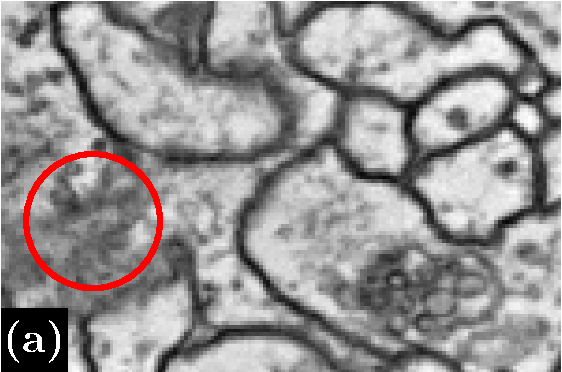
\includegraphics[width=1.0\linewidth,trim=0in 0in 0in 0.2in,clip]{./figs/aff_compare_designer/raw.pdf} % 
% \caption{\centering}
\end{subfigure}\hfill
\begin{subfigure}[t]{0.32\textwidth}
\centering
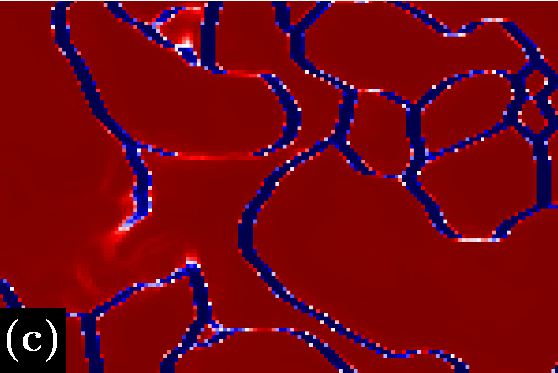
\includegraphics[width=1.0\linewidth,trim=0in 0in 0in 0.2in,clip]{./figs/aff_compare_designer/dice_2.pdf} % ,clip
% \caption{\centering}
\end{subfigure}\hfill
\begin{subfigure}[t]{0.32\linewidth}
\centering
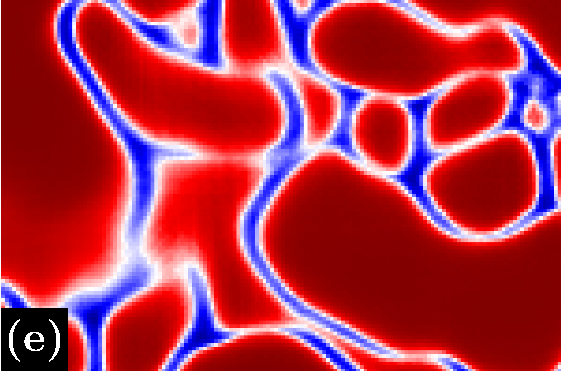
\includegraphics[width=1.0\linewidth,trim=0in 0in 0in 0.2in,clip]{./figs/aff_compare_designer/mask_2.pdf} % ,clip
% \caption{\centering}
\end{subfigure}\vspace{0.6em}\\
\begin{subfigure}[t]{0.32\textwidth}
\centering
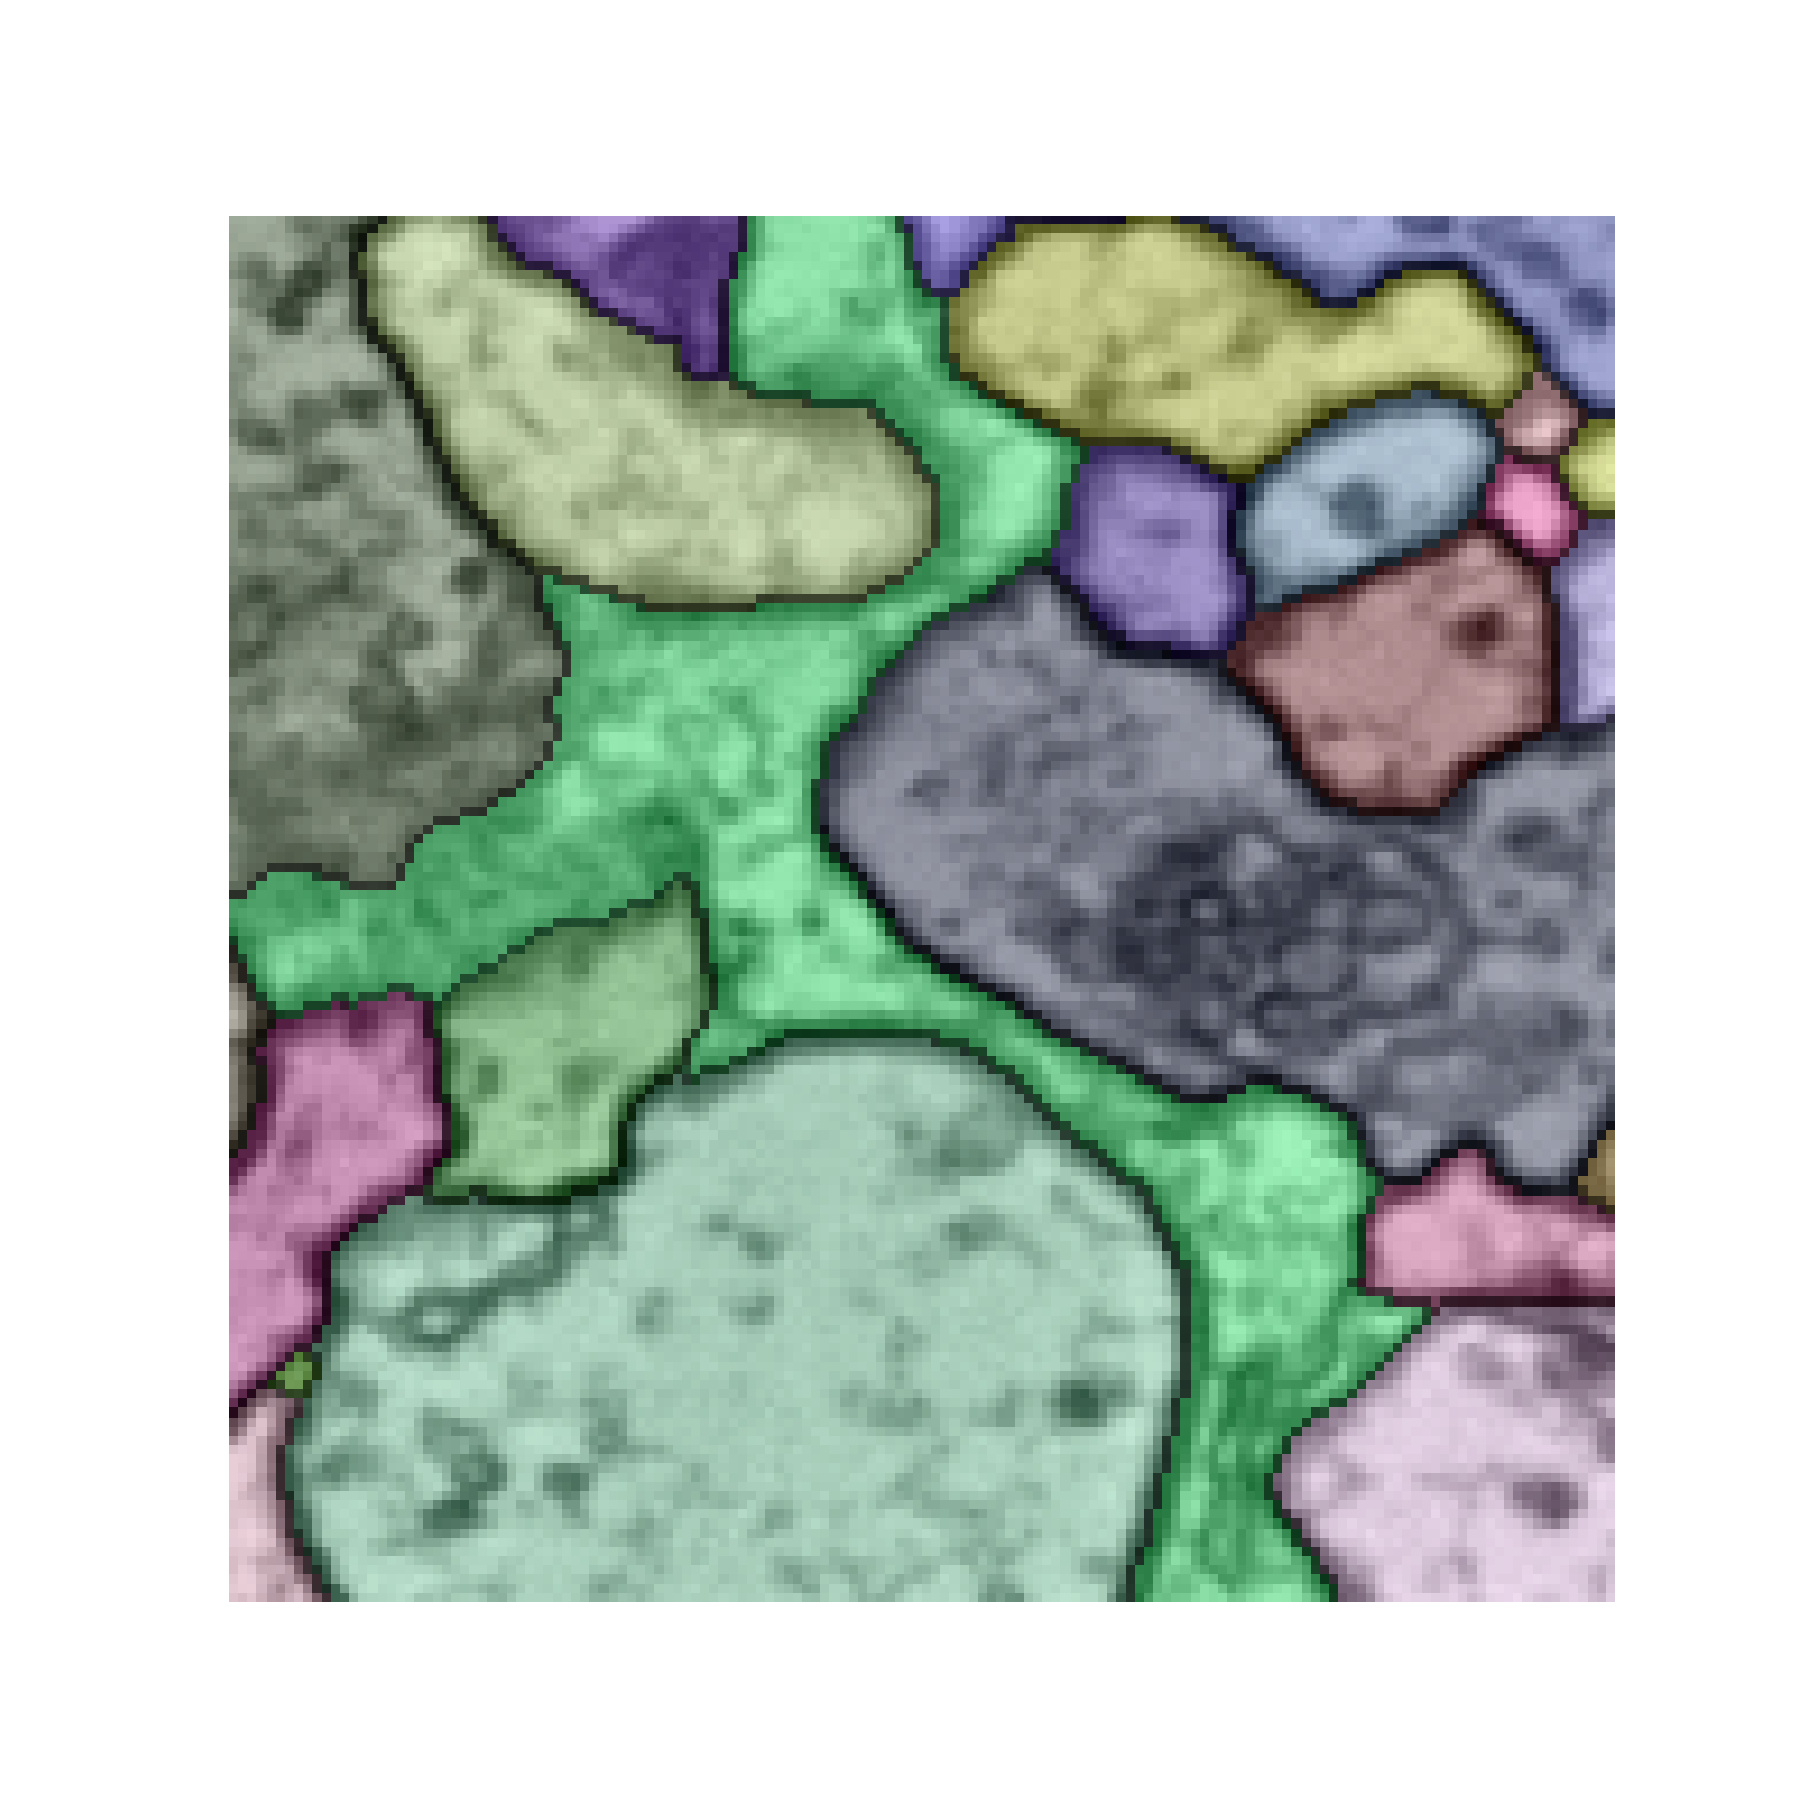
\includegraphics[width=1.0\linewidth,trim=0in 0in 0in 0.2in,clip]{./figs/aff_compare_designer/GT.pdf} % ,clip
% \caption{\centering}
\end{subfigure}\hfill
\begin{subfigure}[t]{0.32\linewidth}
\centering
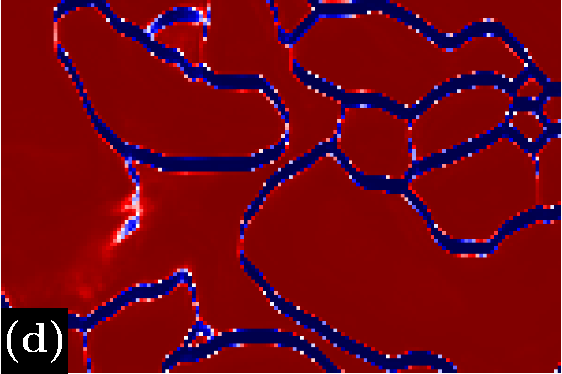
\includegraphics[width=1.0\linewidth,trim=0in 0in 0in 0.2in,clip]{./figs/aff_compare_designer/dice_1.pdf} % ,clip
% \caption{\centering}
\end{subfigure}\hfill
\begin{subfigure}[t]{0.32\textwidth}
\centering
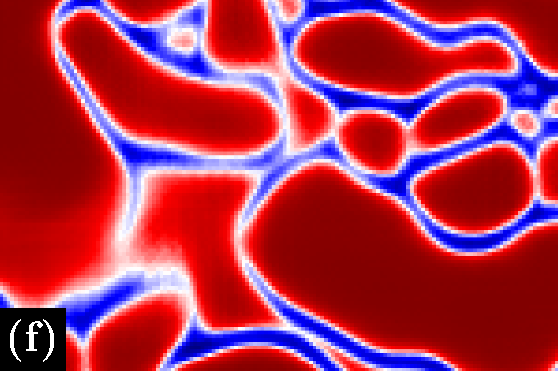
\includegraphics[width=1.0\linewidth,trim=0in 0in 0in 0.2in,clip]{./figs/aff_compare_designer/mask_1.pdf} % ,trim=0.25in 0.25in 0.65in 0.36in,clip
% \caption{\centering}
\end{subfigure}
\caption{Comparison between different affinities and their robustness to noise. \textbf{\mbox{(a-b)}} Raw data and ground-truth labels. \textbf{(c-d)} Affinities predicted by the \emph{sparse-neighborhood branch}, which is trained with a dense binary classification loss (high affinities are represented in red, low ones in blue). \textbf{(e-f)} Affinities computed by averaging overlapping masks as explained in Sec. \ref{sec:aggr_affs} (MaskAggr). We note how affinities from averaged masks are smoother and present a more consistent boundary evidence in the noisy region highlighted by the red circle in \textbf{(a)}. Here we show affinities along the horizontal (-4, 0, 0) and vertical (0, -4, 0) directions.}\label{fig:affs_comparison}
\end{figure}

\subsection{Results and Discussion}

\textbf{Pre-Training of the Encoded Space} -- The proposed model based on an \emph{\encBr branch} can be properly trained only if the dimension $Q$ of the latent space is large enough to accommodate all possible occurring neighborhood patterns. 
To find a small but sufficiently large $Q$, we trained a convolutional Variational Auto-encoder (VAE) \cite{kingma2013auto,rezende2014stochastic} to compress binary ground-truth \maskname masks $\hat{\mathcal{M}}_{\coord{u}}$ into latent variables $z_{\coord{u}}\in \mathbb{R}^Q$ and evaluated the quality of the reconstructed binary masks via the reconstruction loss. We concluded that $Q=32$ is large enough to compress the masks considered here consisting of $7\times 7 \times 5=245$ pixels. 

As a first experiment, we tried to make use of this VAE-pretrained latent space to train the proposed \emph{\encBr branch} and predict encoded masks directly in this space by using an L2 loss on the encoded vectors. However, similarly to the findings of \cite{hirsch2020patchperpix}, this approach performed worse than directly training the full model end-to-end as described in Sec. \ref{sec:encoding_masks}. 
% \begin{itemize}
% \item Mention how we tested the latent space dimension by training a VAE (or AE) to compress binary ground-truth \maskname masks: \emph{We then test this assumption by compressing binary ground-truth \maskname masks $\hat{\mathcal{M}}_{\coord{u}}$ to latent variables $z_{\coord{u}}\in \mathbb{R}^Q$ by training a convolutional Variational Auto-encoder (VAE) \cite{kingma2013auto,rezende2014stochastic} consisting of an encoder $p_{\phi}(z_{\coord{u}}|\hat{\mathcal{M}}_{\coord{u}})$ and a decoder $p_{\phi}(\hat{\mathcal{M}}_{\coord{u}}|z_{\coord{u}})$.
% In our experiments, we evaluate how the dimension $Q$ of the latent space impacts the quality of the reconstructed binary masks and find in this way an optimal latent space dimension that is compact enough but at the same time preserves most of the information contained in the binary masks.}
% \item Mention that we also tried to pre-train the encoded space with a VAE, but this did not work better than directly training the space end-to-end (similarly to PatchPerPix). 
% \emph{In this case, we first train a VAE to encode ground-truth binary masks as explained above in Sec. \ref{sec:encoding_masks}. 
% The main backbone model is then trained to predict, for each pixel $\coord{u}$, the mean and the standard deviation of the encoded distribution $p_{\phi}(z_{\coord{u}}|\hat{\mathcal{M}}_{\coord{u}})$ predicted by the pre-trained encoder, where $\hat{\mathcal{M}}_{\coord{u}}$ is the ground truth \maskname mask associated to pixel $\coord{u}$. An L2 loss is used to pull the two encoded vectors close to each other's. 
% The reasoning behind this approach is to train the backbone model to predict the masks in a meaningful compressed latent space. 
% Nevertheless, as we will show in our experiments, this method was the least successful among the tested ones (\emph{similarly to the findings of \cite{hirsch2020patchperpix}}).}
% \end{itemize}



\textbf{Training Encoded Masks} -- As we show in our validation experiments in Tab. \ref{tab:val_results}, models trained to predict encoded \maskname masks (ENB) achieved better scores than the current state-of-the-art method predicting affinities for a sparse neighborhood structure (SNB). 
% Predicting only affinities for a sparse-neighborhood, like the SBN model, is an easier task as compared to predicting large and dense neighborhood structures. 
Our interpretation of this result is that using the encoding process to predict \maskname masks encourages the model to predict segment shapes that are consistent in a larger neighborhood, which can be helpful to correctly segment the most difficult regions of the data. 
% Thus, we argue that the combined model is less likely to result in a basic boundary detector based on simple local features and it is instead more likely to learn more complex features and use for example prior information about the shape of the segments.
 % like in the models ENB and ENB+SBN, is a more challenging task than predicting affinities for a sparse-neighborhood, like for the SBN model. Thus, we argue that the models predicting \maskname masks are 
 % and instead are encouraged to learn long-range features that can be helpful in the most challenging cases.
% Moreover, ... 
% Not only improves affinities, but also the opposite. 

\begin{table}[t]
% \tiny
\centering
\scriptsize
  % {\renewcommand{\arraystretch}{1.3}
  % \resizebox{\textwidth}{!}{
        \begin{tabular}[t]{c c c c c c c}
         % Method & \makecell{CREMI-Score \\(lower is better)} \\ \midrule 
\makecell{Train \\ Sparse \\Neighbor.\\(SNB)} & \makecell{Train\\ Encoded\\Masks\\(ENB)} & \makecell{Aggregate\\Overlapping\\Masks \\(MaskAggr)} & \makecell{Partitioning \\algorithm} &\makecell{No\\superpixels\\required}  & \makecell{CREMI-Score \\(lower is better)} & \makecell{VI-merge \\(lower is better)} \\ \toprule 

\CrossedBox & \CrossedBox & \CrossedBox & MWS & \CrossedBox & \textbf{0.153} & \textbf{0.272} \\
% \CrossedBox & \HollowBox & \textbf{0.153} & \textbf{0.272} \\
% ENB+SNB+MaskAggr} & \textbf{MWS} & \textbf{0.153} & \textbf{0.272} \\
\HollowBox & \CrossedBox & \CrossedBox & MWS & \CrossedBox & 0.184 & 0.273 \\
\HollowBox & \CrossedBox & \HollowBox & MWS & \CrossedBox & 0.419 & 0.302 \\
\CrossedBox & \CrossedBox & \HollowBox & MWS & \CrossedBox & 0.532 & 0.447 \\
\CrossedBox & \HollowBox & \HollowBox & MWS & \CrossedBox & 1.155 & 0.874 \\ \midrule
\HollowBox & \CrossedBox & \HollowBox & WSDT+GaspAvg & \HollowBox & 0.173 & 0.234 \\
\CrossedBox & \CrossedBox & \HollowBox & WSDT+GaspAvg & \HollowBox & 0.237 & 0.331 \\
\CrossedBox & \HollowBox & \HollowBox & WSDT+GaspAvg & \HollowBox & 0.254 & 0.355 \\
\CrossedBox & \CrossedBox & \CrossedBox & WSDT+GaspAvg & \HollowBox& 0.334 & 0.388 \\
\HollowBox & \CrossedBox & \CrossedBox & WSDT+GaspAvg & \HollowBox & 0.357 & 0.391 \\

% ENB+SNB & MutexWatershed & _affs &  &  &  & 0.585 & 0.257 & 0.454 & 0.878 \\
% SNB & MutexWatershed & _affs &  &  &  & 0.910 & 0.344 & 0.671 & 1.736 \\
% SNB & MutexWatershed & _affs_withLR &  &  &  & 1.126 & 0.487 & 0.766 & 1.837 \\
% ENB & WSDT+MC & 0.178 & 0.040 & 0.233 & 0.557 \\
% ENB+SNB & WSDT+MC & 0.241 & 0.082 & 0.331 & 0.377 \\
% SNB & WSDT+MC & 0.257 & 0.087 & 0.355 & 0.399 \\
% ENB+SNB+MaskAggr & MutexWatershed & _affs &  &  &  & 0.269 & 0.086 & 0.370 & 0.470 \\
% ENB+MaskAggr & MutexWatershed & _affs &  &  &  & 0.302 & 0.095 & 0.365 & 0.595 \\
% ENB+SNB & MutexWatershed & _affs_withLR &  &  &  & 0.416 & 0.145 & 0.385 & 0.803 \\


% % % & & SNB & 1.144 & 0.875 \\ 
% % & & SNB+ENB & \textbf{0.115} & 0.222 \\
% % & & SNB & 0.119 & \textbf{0.219} \\
% % GaspAverage  & & SNB+ENB+MaskAggr &  0.156 & 0.277 \\
% % & &ENB & 0.173 & 0.242 \\
% % & &ENB+MaskAggr & 0.188 & 0.281 \\ \midrule
% & &SNB+ENB & \textbf{0.130} & \textbf{0.234} \\
% WSDT+GaspAverage & & SNB & 0.147 & 0.258 \\
% && ENB & 0.173 & 0.240 \\ \midrule
% & &SNB+ENB & \textbf{0.135} & \textbf{0.235} \\
% WSDT+MC & & SNB &  0.151 & 0.258 \\
% & & ENB & 0.178 & 0.240 \\ \midrule
% & & SNB+ENB+MaskAggr & \textbf{0.155} & 0.278 \\
% & & ENB+MaskAggr & 0.183 & \textbf{0.275} \\
% MutexWatershed & & ENB & 0.417 & 0.311 \\
% & & SNB+ENB &  0.531 & 0.449 \\
% % & & SNB+ENB & 0.539 & 0.376 \\
% & & SNB & 0.895 & 0.634 \\ 
% % Superpixels without long-range:
% % UNet+SNB+ENB & WSDT+GASP-Avg & 0.137 & 0.260 \\
% % UNet+SNB & WSDT+GASP-Avg & 0.188 & 0.333 \\
% % UNet+ENB & WSDT+GASP-Avg & 0.197 & 0.299 \\
% % Multicut without long range:
% % UNet+SNB+ENB & WSDT+MC & 0.127 & 0.245 \\
% % UNet+ENB & WSDT+MC & 0.156 & 0.248 \\
% % UNet+SNB & WSDT+MC & 0.183 & 0.317 \\
% % Superpixels ong MaskAggr
% % UNet+SNB+ENB+MaskAggr & WSDT+GASP-Avg-LR & 0.219 & 0.309 \\
% % UNet+SNB+ENB+MaskAggr & WSDT+GASP-Avg & 0.229 & 0.316 \\
% % UNet+ENB+MaskAggr & WSDT+GASP-Avg-LR & 0.243 & 0.316 \\
% % UNet+ENB+MaskAggr & WSDT+GASP-Avg & 0.248 & 0.323 \\


        \end{tabular}
        % }
        \vspace{1em}
        \caption{Comparison experiments on our CREMI validation set. Training encoded \maskname masks (ENB) achieved better scores than the current state-of-the-art approach training only affinities for a sparse neighborhood (SNB). The model that performed best was the one using the method proposed in Sec. \ref{sec:aggr_affs} to average overlapping masks (MaskAggr).} \label{tab:val_results}
\end{table}


\textbf{Aggregating Overlapping Masks}  -- 
In our validation experiments of Tab. \ref{tab:val_results}, we also test the affinities computed by averaging over overlapping masks (MaskAggr), as described in Sec. \ref{sec:aggr_affs}. We then partition the resulting signed graph by using the Mutex Watershed, which is a very simple parameter-free algorithm with empirical linearithmic complexity in the number of edges. 
Our experiments show that, for the first time on this type of more challenging neuron segmentation data, the Mutex Watershed (MWS) achieves better scores than the super-pixel-based methods (WSDT+GaspAvg), which have so far been known to be more robust to noise but also require the user to tune more hyper-parameters.   

We also note that the MWS achieves competitive scores only with affinities computed from aggregating overlapping masks (MaskAggr).
This shows that the MWS algorithm can take full advantage of the \maskname aggregation process by assigning the highest priority to the edges with largest attractive and repulsive weights that were consistently predicted across overlapping masks.

On the other hand, most of the affinities trained with the \emph{\sparseBr} \linebreak \emph{branch} and a dense binary classification loss are almost binary, i.e. they present values either really close to zero or really close one (see comparison between different types of affinities in Fig. \ref{fig:affs_comparison}).
% In Fig. \ref{fig:affs_comparison} we compare affinities predicted either by averaging \maskname masks or by directly predicting them as a binary classification output of the model trained with a dense channel-wise S\o rensen-Dice loss. 
%\footnote{In practice, this effect is even stronger when the binary classification loss is based on the S\o rensen-Dice coefficient like the one used here.}.
This is not an ideal setup for the MWS, which is a greedy algorithm merging and constraining clusters according to the most attractive and repulsive weights in the graph.
In fact, in this setting the MWS can often lead to over-segmentation and under-segmentation artifacts like those observed in the output segmentations of the (SNB+ENB+MWS) and (SNB+MWS) models. Common causes of these mistakes can be for example inconsistent predictions from the model and partially missing boundary evidence, which are very common in this type of challenging application (see Fig. \ref{fig:affs_comparison} for an example). 
% On the other hand, 
% Thus, we first note that these affinities are substantially different from those computed by averaging over overlapping masks as described in Sec. \ref{sec:aggr_affs} \TODO{Fig?}.
 % This fact is also shown in Table \ref{tab:val_results} by the validation scores achieved by the Mutex Watershed.

Finally, we also note that superpixel-based methods did not perform equally well on affinities computed from aggregated masks and the reason is that these methods were particularly tailored to perform well with the more \emph{binary-like} classification output of the \emph{\sparseBr branch}.


\begin{table}[t]
\centering
\scriptsize
\begin{minipage}[t]{\textwidth}
    \centering
        \begin{tabular}[t]{l c c c c c c}
        Model & \makecell{Train \\ Sparse \\Neighbor.\\(SNB)} & \makecell{Train\\ Encoded\\Masks\\(ENB)} & \makecell{Aggregate\\Overlapping\\Masks \\(MaskAggr)} & \makecell{Partitioning\\algorithm} & \makecell{No\\superpixels\\ required}  & \makecell{CREMI-Score \\(lower is better)}  \\ \midrule
GaspUNet\cite{bailoni2019generalized} & \CrossedBox & \HollowBox & \HollowBox & WSDT+LMulticut & \HollowBox & \textbf{0.221} \\
PNIUNet\cite{lee2017superhuman} & \CrossedBox & \HollowBox & \HollowBox & Z-Watershed+Agglo & \HollowBox & 0.228 \\
GaspUNet\cite{bailoni2019generalized} & \CrossedBox & \HollowBox & \HollowBox & GaspAvg & \CrossedBox & 0.241  \\
\textbf{OurUNet} & \CrossedBox & \CrossedBox & \CrossedBox &MWS & \CrossedBox & 0.246  \\
\textbf{OurUNet} & \HollowBox & \CrossedBox & \HollowBox &  WSDT+GaspAvg  & \HollowBox & 0.268  \\
MALAUNet\cite{funke2018large} & \CrossedBox & \HollowBox & \HollowBox & WSDT+Multicut & \HollowBox & 0.276  \\
\textbf{OurUNet} & \CrossedBox & \CrossedBox & \HollowBox & WSDT+GaspAvg & \HollowBox & 0.280  \\
CRUNet\cite{zeng2017deepem3d} & \HollowBox & \HollowBox & \HollowBox & 3D-Watershed & \HollowBox & 0.566   \\
LFC\cite{parag2017anisotropic} & \CrossedBox & \HollowBox & \HollowBox & Z-Watershed+Agglo & \HollowBox & 0.616  \\
        \end{tabular}
        \vspace*{0.99em}
    \caption{Representative excerpt of the published methods currently part of the CREMI leaderboard \cite{cremiChallenge} (March 2020). The best method proposed in this work achieves competitive scores and is based on an efficient parameter-free algorithm that does not rely on superpixels. For more details about the partitioning algorithms used by related work, see references in the first column.}
    \label{tab:test_results}
\end{minipage}
\end{table}

% \begin{table}[t]
% \centering
% \scriptsize
% \begin{minipage}[t]{\textwidth}
%     \centering
%         \begin{tabular}[t]{L{18em} c M{8.7em} c}
%         Model & \makecell{Partitioning\\algorithm} & \makecell{CREMI-Score \\(lower is better)} & \makecell{No superpixels\\ required}  \\ \midrule
% GaspUNet+SNB+EffAff \cite{bailoni2019generalized} & WSDT+LMC  &  0.221 & \HollowBox \\
% PNIUNet+SNB+EffAff \cite{lee2017superhuman} & Z-Watershed+Agglo  & 0.228 & \HollowBox \\
% GaspUNet+SNB+EffAff \cite{bailoni2019generalized} & GaspAvg & 0.241 & \CrossedBox \\
% \textbf{OurUNet+ENB+SNB+MaskAggr} &\textbf{MWS} & \textbf{0.246} & \CrossedBox \\
% OurUNet+ENB+EffAff& WSDT+GaspAvg  & 0.268 & \HollowBox \\
% MALAUNet+EffAff \cite{funke2018large} & WSDT+Multicut  & 0.276 & \HollowBox \\
% OurUNet+ENB+SNB+EffAff & WSDT+GaspAvg & 0.280 & \HollowBox \\
% CRUNet \cite{zeng2017deepem3d} & 3D-Watershed & 0.566  & \HollowBox \\
% LFC+EffAff \cite{parag2017anisotropic} & Z-Watershed+Agglo & 0.616  & \HollowBox \\
%         \end{tabular}
%         \vspace*{0.99em}
%     \caption{Representative excerpt of the published methods currently part of the CREMI leaderboard \cite{cremiChallenge} (March 2020). The best method proposed in this work (highlighted in bold) achieves competitive scores and is based on an efficient parameter-free algorithm that does not rely on superpixels.}
%     \label{tab:test_results}
% \end{minipage}
% \end{table}



\textbf{Training Both Masks and a Sparse Neighborhood} -- In our validation experiments, the combined model, which was trained to predict both a sparse neighborhood (SNB) and encoded \maskname masks (ENB), achieved the best scores and yielded sharper and more accurate mask predictions.
In general, providing losses for multiple tasks simultaneously has often been proven beneficial in a supervised learning setting.
Moreover, the dense gradient of the \emph{\encBr branch}, which focuses on locally correct predictions, nicely complements the sparse gradient\footnote{The gradient of the \emph{\encBr branch} is sparse, due to GPU-memory constraints as explained in Sec. \ref{sec:encoding_masks}.} of the \emph{\encBr branch}, which focuses on predictions that are consistent in a larger neighborhood. We expect this to be another reason why the combination of affinities and \maskname masks performed best in our experiments. 
% In our case, the better performances of the combined model could also be explained by the fact that, due to GPU-memory restrictions, the \emph{\encBr branch} was trained only with a sparse gradient from a small fraction of all the predicted encoded masks (see Sec. \ref{sec:encoding_masks}), whereas the \emph{\sparseBr branch} received gradient for every pixel in the output feature map. \\
% On the other hand, the combined model ENB+SNB, which receives dense gradient from the \emph{\sparseBr branch}, predicted sharper and more accurate \maskname mask as compared to the ENB model. Thus, to summarize, our results show that the combined model trained to predict both affinities and \maskname masks performs better than the models trained to solve the two tasks singularly, which is a common behavior often observed in supervised learning. \\





\textbf{Results on Test Samples} -- The evaluation on the three test samples presented in Tab. \ref{tab:test_results} confirms our findings from the validation experiments: among the methods tested in this work, the best scores are achieved by the combined model (ENB+SNB) and by using the Mutex Watershed algorithm (MWS) on affinities averaged over overlapping masks (MaskAggr).
Our method achieves comparable scores to the only other method in the leader-board that does not rely on super-pixels (line 3 in Table \ref{tab:test_results}). This method uses the average agglomeration algorithm GaspAvg proposed in \cite{bailoni2019generalized} instead of the MWS. GaspAvg has been shown to be more robust to noise than Mutex Watershed, however it is also considerably more computationally expensive to run on large graphs like the ones considered here. 

% The other leading entries in the leaderboard are all given by methods that are very similar to our baseline model SNB, which in our validation experiments consistently performed worse.
% A possible explanation of this result could be that all our trained models seem to suffer particularly from the \emph{glia-confusion problem}, that has been already observed in related work on neuron segmentation \TODO{\cite{lee2019learning,januszewski2018high}}. Glia (putative astrocyte) are segments that look quite different from other neurons and are usually considered separately in the final reconstructed diagram of neural circuit connectivity. They often present a main body with a lot of very thin processes that can be \emph{self-touching}. 
% % glia segments are substantially different from the other neurons and are usually considered separately in the final reconstructed diagram of neural circuit connectivity. Glia segments usually present a main body with a lot of very thin glial processes
% Locally, at these self-touching points, glial thin fragments look like distinct segments with clear membrane evidence separating them, even though in the full 3D volume they are connected and hence share the same ground truth label.
% When this happens during training, the model is initially confused and then usually tries to ``memorize'' these self-touching examples by predicting high affinity values despite the clear membrane evidence.
% % When these self-touching examples happen on the training set, despite the clear neuron membrane evidence, the model is trained to predict the same 
% % Every time there is a glia fragment in the training dataset presents two narrow processes that are self-touching, the model is trained to predict one single label for them, even though these processes locally appear like two distinct neurons with clear membrane evidence separating them.
% In practice, this can often lead to wrong merge decisions on the validation and test set, because the model confuses distinct narrow neurons for self-touching fragments of the same glia and wrongly predicts a high merge-affinity connecting them.
% In future work, we plan to process this type of glial fragments differently, similarly to related work \TODO{\cite{lee2019learning,januszewski2018high}}. 





